\chapter{XML Schemas}

\section{DTD vs XSD}
\begin{itemize}
\item XML Schema (XSD) is itself an XML language. DTDs (a relict from SGML times) use a different syntax.
\item DTDs do not fully support namespaces; XML Schema does.
\item XML Schema allows validation of element and attribute content against built-in or user-defined data types.
\item With XML Schemas we can more easily create complex and reusable structures and types.
\item HTML is not XML and therefore still needs a DTD. Other than that I believe that DTDs are dying out.
\end{itemize}

\begin{lstlisting}[language=XML, caption={DTD Example}]
<!DOCTYPE NEWSPAPER [
<!ELEMENT NEWSPAPER (ARTICLE+)> <!ELEMENT ARTICLE (HEADLINE, BYLINE, LEAD, BODY, NOTES)> <!ELEMENT HEADLINE (#PCDATA)> <!ELEMENT BYLINE (#PCDATA)> <!ELEMENT LEAD (#PCDATA)> <!ELEMENT BODY
(#PCDATA)> <!ELEMENT NOTES (#PCDATA)>
<!ATTLIST ARTICLE AUTHOR CDATA #REQUIRED>
<!ATTLIST ARTICLE EDITOR CDATA #IMPLIED> <!ATTLIST ARTICLE DATE CDATA #IMPLIED> <!ATTLIST ARTICLE EDITION CDATA #IMPLIED> <!ENTITY NEWSPAPER "Vervet Logic Times"> <!ENTITY PUBLISHER "Vervet Logic Press"> <!ENTITY COPYRIGHT "Copyright 1998 Vervet Logic Press">]>
\end{lstlisting}

\section{Three good Reasons for XML Schemas}
Regel: \red{\textbf{Wir lesen niemals XML Dokumente ein, ohne sie zu validieren!}}
\begin{enumerate}
\item An XML processing application can validate an input file against a Schema using a standard parser. This directly separates out incorrect files. Syntax checking of input files reduces to typing 3 lines of code. This is cheap, fast and produces less software bugs.
\item If you need to specify a new data exchange format with your business partners, write an XML Schema. This provides specification, documentation and validator at once.
\item Object-oriented programming languages such as Java or C\# directly allow to construct type hierarchies from XML Schemas. The same works with XML databases.
\end{enumerate}

\section{Validating XML Files against XML Schemas}
\begin{itemize}
\item If an XML document adheres an XML Schema, it is called an instance of this Schema.
\item It is possible to directly embed a Schema definition into an XML document (e.g. if the document will remain the only instance), but most of the time Schemas are in separate files.
\item There are different ways of how to validate an XML document:
\begin{enumerate}
\item Online Schema Validator, e.g. \href{http://www.corefiling.com/opensource/schemaValidate.html}{http://www.corefiling.com/opensource/schemaValidate.html} 
\item IDEs such as NetBeans have built-in validators
\item Use a parser in your favourite programming language
\end{enumerate}
\end{itemize}

\section{Exercise: Validation}

\section{XML Namespaces vs Java Packages}
\begin{enumerate}
\item XML Schemas define new XML languages or vocabularies comparable to e.g. packages in Java defining new API
\item If a class belongs to a package in Java, then this package is declared in the source code and must be imported for usage
\item Putting a class into a package in Java is not mandatory.
Likewise, putting a vocabulary into a namespace is not mandatory.
\item In the same way, if some vocabulary is part of a namespace, this namespace must be declared in the source code (XML Schema) and imported for usage (XML document)
\item A namespace assigned to a Schema is called target namespace
\end{enumerate}

\section{Example: Target Namesapce for SVG}
\begin{itemize}
\item We already saw that the namespace for SVG is
http://www.w3.org/2000/svg
This namespace is set inside the XML Schema for SVG as target namespace, check yourself:
http://www.w3.org/TR/2002/WD-SVG11-20020108/SVG.xsd
\item By the way, this is how a browser identifies SVG code and applies language specific rendering instead of a default action.
\item Most browsers have a built-in, hard-coded list of namespaces with specialized rendering, e.g. for XHTML, SVG, MathML, RSS, ...
\end{itemize}

\section{Do I need a target namesapce?}

\begin{itemize}
\item No, just refer in your XML document to an XML schema, and your code can be validated. In fact, we will do without target namespaces for most of our simple examples
\item Sometimes your XML Schema is distributed over multiple files. Then, using a target namespace, you can signal that all this vocabulary belongs to the same language.
\item If you want to combine several vocabularies in the same document (e.g. mix bond movies with country information) there can be at most one vocabulary without a target namespace.
\item Web languages like XHTML, SVG and MathML are often combined in the same document. Fortunately, they all have target namespaces.
\end{itemize}


\section{Binding without Target Namespace 1}
If the XML Schema does not define a target namespace for its vocabulary, the binding works as follows:
\begin{lstlisting}[language=XML, caption={Binding without Target Namespace 1}]
<european_countries 
	xmlns:xsi="http://www.w3.org/2001/XMLSchema-instance"
	xsi:noNamespaceSchemaLocation="countries_without_targetns.xsd"
	year="1999">
	<country>
		<name>Switzerland</name> <population>7124000</population>
		<population_under_15>17.5</population_under_15> 
		<population_over_64>15.2</population_over_64> 
		<life_exp_men>76.5</life_exp_men> <life_exp_women>82.5</life_exp_women>
	</country> ...
</european_countries>
\end{lstlisting}

\section{Binding without Target Namespace 2}
\begin{itemize}
\item The attribute value is the path or URL to the XML Schema file. \item This just points at the definition of the vocabulary and imports
all definitions from the referenced Schema.
\item The attribute noNamespaceSchemaLocation for binding an XML file to a Schema without target namespace belongs to the XML Schema language, i.e. it is part of the target namespace
http://www.w3.org/2001/XMLSchema-instance
Therefore we must import this namespace as well.
\end{itemize}

\section{Binding with Target Namespace 1}
If the XML Schema is supposed to define the target namespace \red{http://www.marcpouly.ch/countries} for its vocabulary,
the binding works as follows:
\begin{lstlisting}[language=XML, caption={Binding with Target Namespace 1}]
<european_countries 
	year="1999" 
	xmlns="http://www.marcpouly.ch/countries" 
	xmlns:xsi="http://www.w3.org/2001/XMLSchema-instance"
	xsi:schemaLocation="http://www.marcpouly.ch/countries countries_with_targetns.xsd">
	<country>
		<name>Switzerland</name> 
		<population>7124000</population> 
		<population_under_15>17.5</population_under_15> 
		<population_over_64>15.2</population_over_64> 
		<life_exp_men>76.5</life_exp_men> 
		<life_exp_women>82.5</life_exp_women>
	</country> ...
</european_countries>
\end{lstlisting}

\section{Binding with Target Namespace 2}
\begin{itemize}
\item The attribute schemaLocation for binding an XML file to a Schema with target namespace belongs to the XML Schema namespace.
\item The attribute value now is a list of namespace-location pairs separated by whitespace. The location specifies where the Schema can be found and which target namespace belongs to which Schema.
\item This imports everything that belongs to the target namespace http://www.marcpouly.ch/countries from the given XSD file.
\item We further declare http://www.marcpouly.ch/countries as default namespace because the majority of the used elements belong to this namespace (we could also use a prefix of course).
\end{itemize}
\begin{lstlisting}[language=XML, caption={Binding with Target Namespace 2}]
<european_countries 
	year="1999" 
	xmlns="http://www.marcpouly.ch/countries" 
	xmlns:xsi="http://www.w3.org/2001/XMLSchema-instance"
	xsi:schemaLocation="http://www.marcpouly.ch/countries 
	countries_with_targetns.xsd">
	<country>
		<name>Switzerland</name> 
		<population>7124000</population> 
		<population_under_15>17.5</population_under_15> 
		<population_over_64>15.2</population_over_64> 
		<life_exp_men>76.5</life_exp_men> 
		<life_exp_women>82.5</life_exp_women>
	</country> ...
</european_countries>
\end{lstlisting}

\section{XML Schema Skeleton without Target Namespace}
\begin{lstlisting}[language=XML, caption={XML Schema Skeleton without Target Namespace}]
<?xml version="1.0"?>
<xs:schema xmlns:xs="http://www.w3.org/2001/XMLSchema">
	<!-- Schema content --> 
</xs:schema>
\end{lstlisting}
\begin{itemize}
\item Because we want to use the XML Schema language we must declare the XML Schema namespace.
\item I strongly recommend to always use a prefix for the XML Schema namespace. As you define your own language elements in a Schema, parsers must be able to distinguish the two languages. We will illustrate the problems occurring without prefix later.
\end{itemize}

\section{Skeleton Extension for Target Namespace}
\begin{lstlisting}[language=XML, caption={Skeleton Extension for Target Namespace}]
<xs:schema xmlns:xs="http://www.w3.org/2001/XMLSchema"
	xmlns="http://www.marcpouly.ch/countries"
	targetNamespace="http://www.marcpouly.ch/countries" 
	elementFormDefault="qualified">
	<!-- Schema content --> 
</xs:schema>
\end{lstlisting}
\begin{itemize}
\item We further define the target namespace using the XML Schema attribute targetNamespace and also set this namespace as default
namespace for the XML Schema (we could also use a prefix).
\item We qualify all elements with elementFormDefault="qualified" in order to automatically put all elements into the target namespace (see next slide).
\end{itemize}

\section{Qualified Elements and Attributes}
\begin{itemize}
\item An element or attribute is called qualified if it belongs to a namespace.
\item By adding elementFormDefault="'qualified"' we signal that by default
all elements belong to the target namespace. The default value of this attribute is unqualified.
\item By adding \code{attributeFormDefault="'qualified"'} (default is unqualified) we would signal that attributes can be combined with elements from other languages, e.g. noNamespaceSchemaLocation from the XML Schema namespace is used inside \code{<european\_countries>}.
\item We will talk about this later again and also illustrate that in such cases we cannot work with default namespaces in instance documents anymore. Instead, we must give a prefix to every qualified attribute.
\end{itemize}

\section{Simple Elements}
\begin{lstlisting}[language=XML, caption={Simple Elements}]
<xs:element name="name" type="xs:string"/>
<xs:element name="population" type="xs:positiveInteger"/>
<xs:element name="life_exp_women" type="xs:decimal"/>
\end{lstlisting}
\begin{itemize}
\item These elements are atomic because they do not contain sub\item elements. Their content is an XML Schema simple data type.
\item Note the use of the namespace prefix here. Because <element> is prefixed, the parser can deduce that the attributes are those of
this element. However, this does not hold for the attribute values. Therefore, the simple data types has to be prefixed too.
\end{itemize}

\section{Simple Data Types}
\begin{figure}[h!]
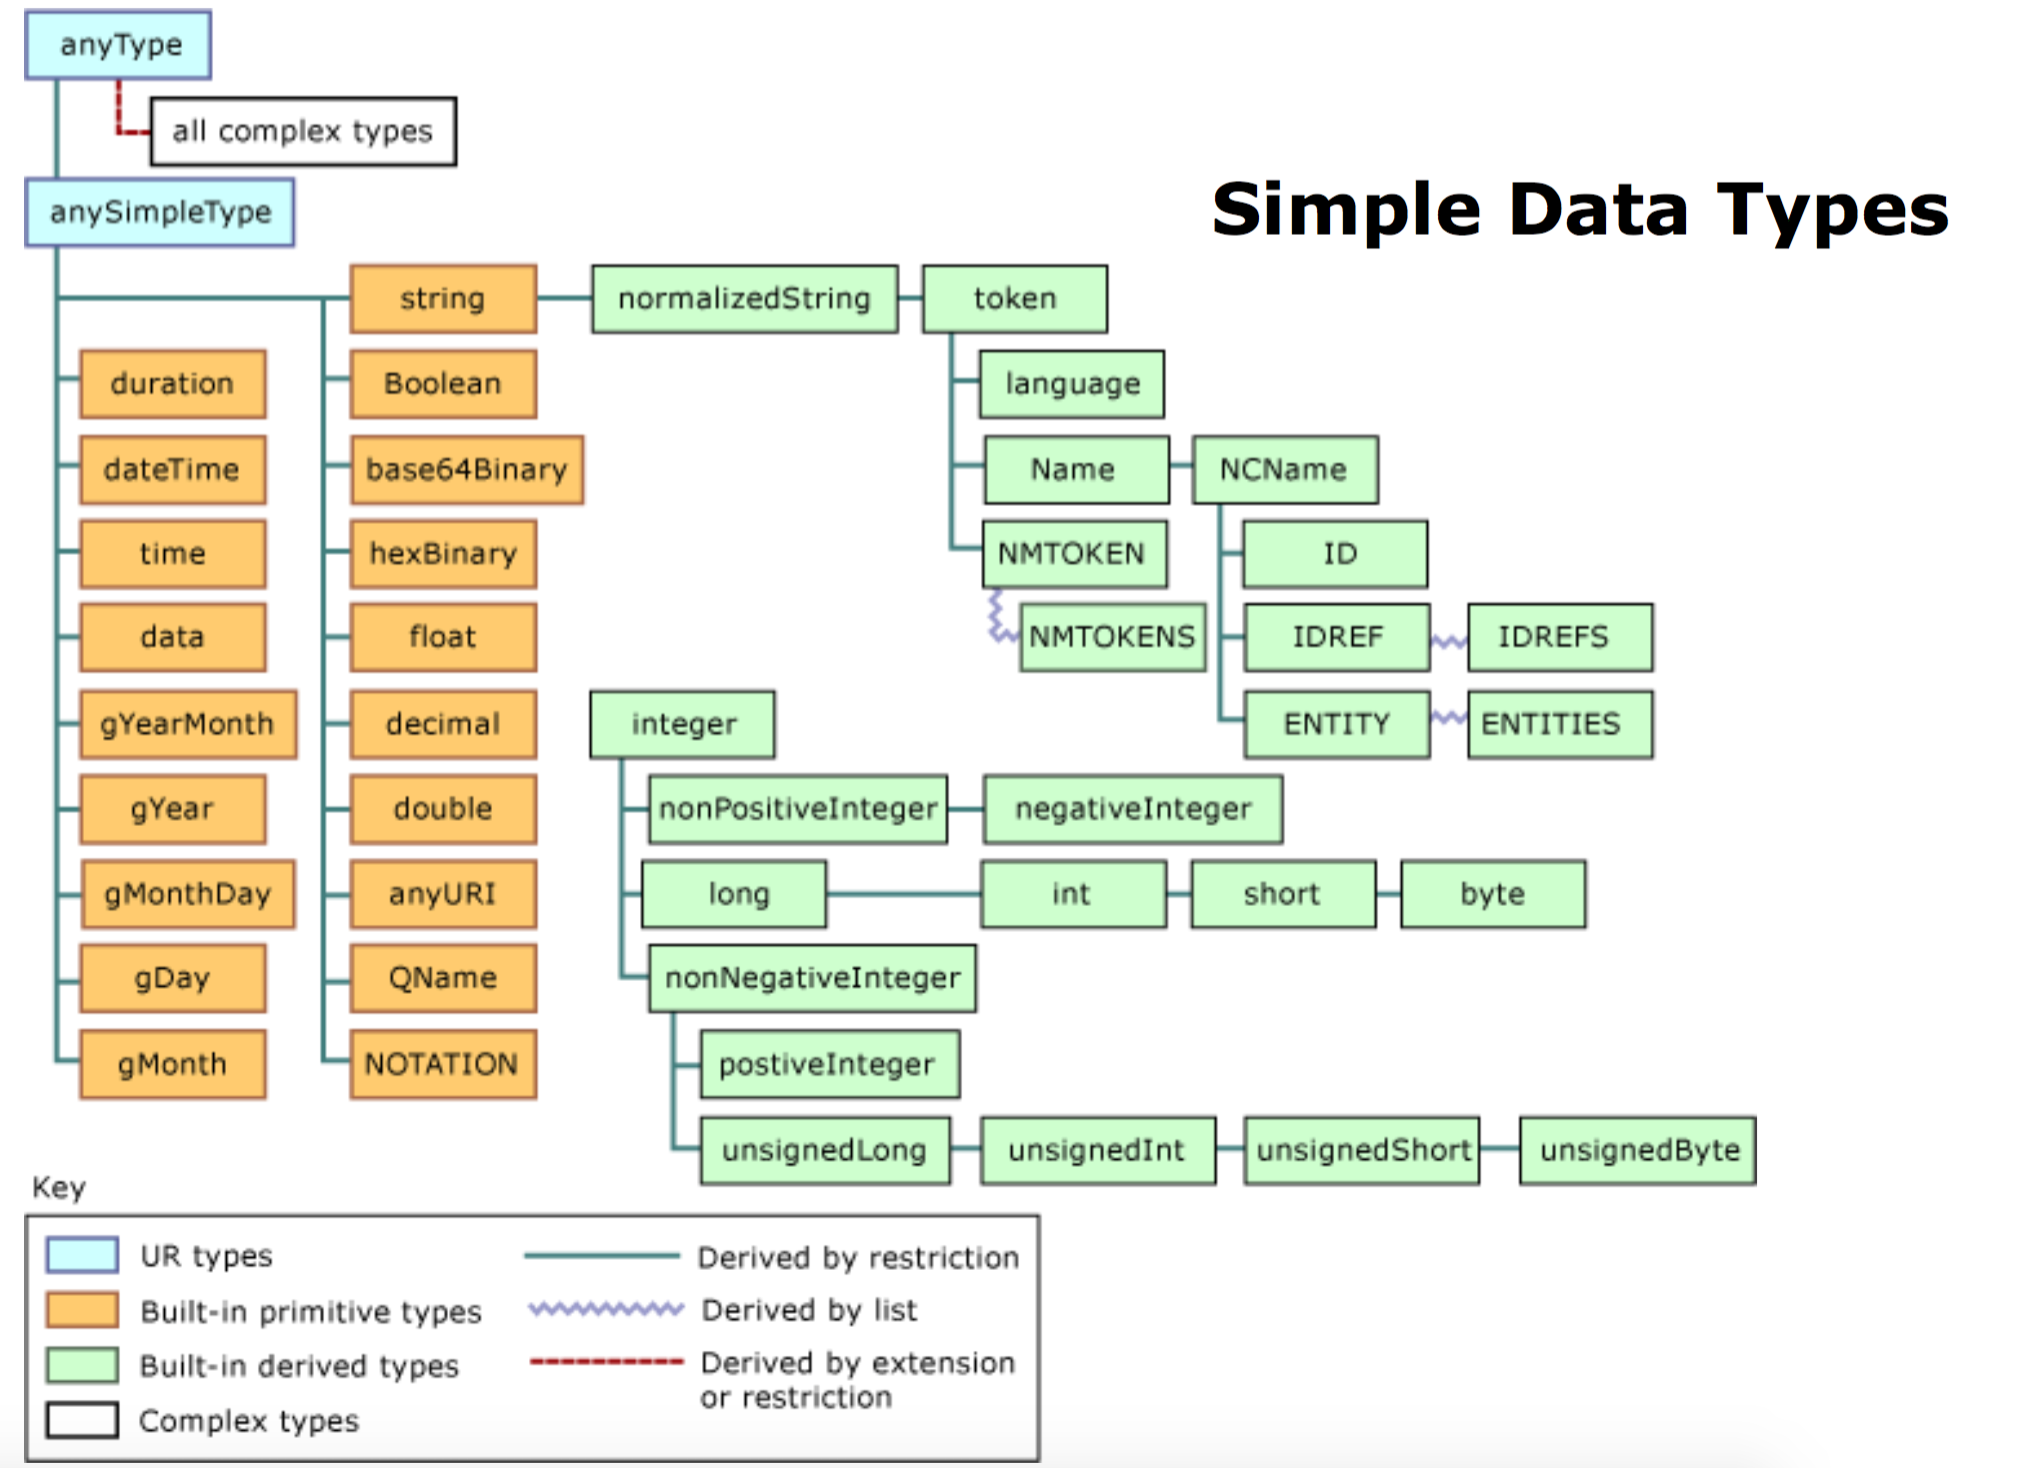
\includegraphics[width=\textwidth]{fig/SimpleDataTypes.png}
\end{figure}

\section{New Simple data Types by Restricition 1}
\begin{lstlisting}[language=XML, caption={Simple Elements}]
<xs:element name="population_under_15" type="percentType"/>
<xs:simpleType name="percentType"> 
	<xs:restriction base="xs:decimal">
		<xs:minInclusive value="0"/>
		<xs:maxInclusive value="100"/>
	</xs:restriction>
</xs:simpleType>
<xs:simpleType name="beer"> 
	<xs:restriction base="xs:string">
		<xs:enumeration value="Cardinal"/> 
		<xs:enumeration value="Lozaerner Bier"/> 
		<xs:enumeration value="Eichhof"/> 
		<xs:enumeration value="Boxer"/>
	</xs:restriction> 
</xs:simpleType>
\end{lstlisting}

\section{Constraints for Restrictions}
BIld hier einfügen

\section{Building Complex Types}
\begin{itemize}
\item Complex elements may contain sub-elements:
\begin{itemize}
\item <sequence> elements must appear in the given order,
\item <choice> if exactly one element is to be selected,
\item <all> elements can appear zero or one time in any order.
\end{itemize}
\item Complex elements may contain attributes.
\item Remember that an attribute is not a sub-element but an integral part. Therefore, even if an element only contains an attribute and nothing else, it is called complex type.
\end{itemize}

\section{Sequences with Local Definitions}

\begin{lstlisting}[language=XML, caption={Sequences with Local Definitions}]
<xs:element name="pets">
	<xs:complexType>
		<xs:sequence minOccurs="0" maxOccurs="unbounded">
			<xs:element name="dog" type="xs:string"/>
      		<xs:element name="cat" type="xs:string"/>
		</xs:sequence>
 	</xs:complexType>
</xs:element>
\end{lstlisting}
\red{\textbf{REIHENFOLGE MUSS SEIN: Zuerst alle Hunde, dann alle Katzen auflisten.}}

\section{Sequences with Global Definitions}
\begin{lstlisting}[language=XML, caption={Sequences with Global Definitions}]
<xs:element name="european_countries">
	<xs:complexType>
		<xs:sequence minOccurs="1" maxOccurs="unbounded">
			<xs:element ref="country"/>
		</xs:sequence>
	</xs:complexType>
</xs:element>
\end{lstlisting}
\begin{itemize}
\item At least one sub-element of type <country>.
\item If element <country> is defined globally it can be referenced.
\end{itemize}

\section{Choices}
Ist entweder-oder.
\begin{lstlisting}[language=XML, caption={Sequences with Global Definitions}]
<xs:element name="person">
	<xs:complexType>
		<xs:choice>
			<xs:element name="employee" type="xs:string"/>
			<xs:element name="player" type="xs:string"/>
		</xs:choice>
	</xs:complexType>
</xs:element>
\end{lstlisting}
\begin{itemize}
\item Casino employees are not supposed to play. A person in a casino must therefore either be an employee or a player (but not both).
\end{itemize}

\section{Sets}
\begin{lstlisting}[language=XML, caption={Sequences with Global Definitions}]
<xs:element name="country">
	<xs:complexType>
		<xs:all>
			<xs:element name="name" type="xs:string"/>
			<xs:element name="population" type="xs:positiveInteger"/>
		</xs:all> 
	</xs:complexType>
</xs:element>
\end{lstlisting}

The global definition of <country> could look like this. It must have exactly one element of type <name> and <population> in any order. We can change this to at most one as follows:

\begin{lstlisting}[language=XML, caption={Sequences with Global Definitions}]
<xs:element name="country">
	<xs:complexType>
		<xs:all minOccurs="0">
			<xs:element name="name" type="xs:string"/>
			<xs:element name="population" type="xs:positiveInteger"/>
		</xs:all>
	</xs:complexType>
</xs:element>
\end{lstlisting}


\section{Combining Complex Types}
Sequences and choices can contain elements that are complex types themselves. Sets (\code{<all>}) cannot. Also, sets cannot be combined
with other complex types as component of a complex type.
\begin{lstlisting}[language=XML, caption={Sequences with Global Definitions}]
<xs:complexType name="NameOrEmail">
	<xs:choice>
		<xs:element name="email" type="xs:string"/>
		<xs:sequence>
			<xs:element name="first" type="xs:string"/>
			<xs:element name="last" type="xs:string"/>
		</xs:sequence>
	</xs:choice>
</xs:complexType>
\end{lstlisting}

A global definition of a type (reusable by different elements) that can either be an email address or first and last name.\\
\red{\code{<all>}} cannot be used in this way !

\section{Simple Elements with Attributes}
What we want ...

\code{<product price="'2.00"'>Coffee in HSLU canteen</product>}\\
An element with simple (string) content and one (decimal) attribute. An element with attributes is a complex type (cf. slide 23).\\
\red{Do not confuse type with content !}
\begin{lstlisting}[language=XML, caption={Sequences with Global Definitions}]
<xs:element name="product">
	<xs:complexType>
		<xs:simpleContent>
			<xs:extension base="xs:string">
				<xs:attribute name="price" type="xs:decimal" />
			</xs:extension>
		</xs:simpleContent>
	</xs:complexType>
</xs:element>
\end{lstlisting}

\section{Attribute as Local Definition}
\begin{lstlisting}[language=XML, caption={Sequences with Global Definitions}]
<xs:element name="european_countries">
	<xs:complexType>
		<xs:sequence minOccurs="1" maxOccurs="unbounded"> 
			<xs:element ref="country"/>
		</xs:sequence>
		<xs:attribute name="year" type="xs:gYear" use="required"/>
	</xs:complexType>
</xs:element>
\end{lstlisting}
"`required"' bedeutet, dass das Attribut hier sein muss.
\begin{itemize}
\item Attribute values are restricted to simple types.
\item Attributes are optional by default unless use="'required"'
\item Attributes with default value:

\code{<xs:attribute name="language" type="xs:string" default="EN"/>}
\end{itemize}

\section{Attribute as Global Definition}
\textbf{Q}: Can I define and reference global attributes ?\\\\
\textbf{A}: Yes, but I do not recommend.\\

The XML Schema specification enforces that global elements or attributes must be qualified, i.e. belong to a namespace. For elements this is no problem. For qualified attributes, however, you cannot work with default namespaces in your instance document anymore.\\
Remember, even if an element belongs to a namespace, its attributes do not automatically belong to it. With qualified attributes you have to give them an explicit prefix. This is the same problem as with attributeFormDefault="qualified" in the root element.


\section{Additional Schema Features: Mixed Content}

\section{Additional Schema Features: Wildcards}
Eine Wildcard ist irgendeine 
\begin{lstlisting}[language=XML, caption={Sequences with Global Definitions}]
<xs:element name="catalogue"> 
	<xs:complexType>
		<xs:sequence>
			<xs:element name="Book" maxOccurs="unbounded">
				<xs:complexType>
					<xs:sequence>
						<xs:element name="Title" type="xs:string"/> 
						<xs:element name="Author" type="xs:string"/> 
						<xs:any namespace="##any" minOccurs="0"/>
					</xs:sequence>
				</xs:complexType>
			</xs:element>
		</xs:sequence>
	</xs:complexType>
</xs:element>
\end{lstlisting}

After \code{<Author>} \red{one} other well-formed XML element from any namespace \red{may} come. With the namespace attribute one may define from which namespace the unknown element is allowed to come in.

\section{Unique Particle Attribution}
\begin{lstlisting}[language=XML, caption={Sequences with Global Definitions}]
<xs:element name="catalogue"> 
	<xs:complexType>
		<xs:sequence>
			<xs:element name="Book" maxOccurs="unbounded">
				<xs:complexType>
					<xs:sequence>
						<xs:element name="Title" type="xs:string"/> 
						<xs:element name="Author" type="xs:string" minOccurs="0"/> 
						<xs:any namespace="##any" minOccurs="0"/>
					</xs:sequence>
				</xs:complexType>
			</xs:element>
		</xs:sequence>
	</xs:complexType>
</xs:element>
\end{lstlisting}
Es ist nun nicht klar, nach welchem Tag (Author oder \code{<any>}) der Code validiert wird $\rightarrow$ schwierig für Parser.

\section{Additional Schema Features: Lists}
In XML Schema:
\begin{lstlisting}[language=XML, caption={Sequences with Global Definitions}]
<xs:simpleType name="monthType"> 
	<xs:restriction base="xs:string">
		<xs:enumeration value="January"/> 
		<xs:enumeration value="February"/> 
		...
		<xs:enumeration value="December"/> 
	</xs:restriction>
</xs:simpleType>

<xs:element name="months">
	<xs:simpleType>
		<xs:list itemType="monthType"/>
	</xs:simpleType>
</xs:element>
\end{lstlisting}

\section{Additional Schema Features: Uniqueness 1}

\begin{lstlisting}[language=XML, caption={Sequences with Global Definitions}]
<xs:element name="bond_movies"> 
	<xs:complexType>
		<xs:sequence>
			<xs:element ref="movie" minOccurs="1" maxOccurs="unbounded"/>
		</xs:sequence>
		<xs:attribute name="month" type="monthType" use="required"/> 
		<xs:attribute name="year" type="xs:gYear" use="required"/>
	</xs:complexType>
	
	<xs:unique name="movieID"> 
		<xs:selector xpath="movie"/> 
		<xs:field xpath="@number"/>
	</xs:unique>
</xs:element>
\end{lstlisting}

\section{Additional Schema Features: Key References}
Referenzieren ist auch möglich. durch das \code{refer} Schlüsselwort wird sichergestellt, dass auf ein existierenden Key verwiesen wird.





\section{Control Questions A}
\begin{enumerate}
\item Unterschied Wohlgeformt und gültig.
\begin{itemize}
\item Wohlgeformt: Hat keine komischen Verschachtelungen USW
\item gültig: Entspricht einem Schema
\end{itemize}

\item Vorteile XML über DTD:
\begin{itemize}
\item Vererbung gibt es nicht in DTD
\item Keine Namespaces
\item Keine Enumerationen
\end{itemize}

\item Wann benötigt man ein XML Schema?\\
Spätestens wenn man ein XML Dokument benötigt (Schreibt oder liest).

\item Target Namespace\\
Man definiert einen Namen für seine eigene XML-Sprache.

\item Was bedeutet es, ein Element zu qualifizieren?\\
Der Target Namespace definiert den Namen seiner Sprache. Aber im XML kann man 

\item Was ist der Unterschied zwischen \code{<all>} und \code{<sequence>} und \code{<choice>}?\\
\code{<all>} muss alle enthalten ohne Reihefolge zu beachten, \code{<sequence>} beachtet reihenfolge und \code{<choice>} ist Mutual Exclusive (entweder oder).

\item Extension und Restriction\\
Extension macht zusätzliche Attribute möglich, Restriction bedeutet \textbf{nicht}, dass man Attribute löschen kann, aber man kann sie einschränken.

\item Automatische Typsubstitution von XML-Schema im vgl. zu Java:\\
Java kann man ein Interface definieren, vom Typ \code{Car} und dann kann man eine Klasse erstellen, die von \code{Car} ableitet und z.B. \code{BMW} heisst.
Erstellt man nun ein Array vom Typ \code{Car}, kann man ein Objekt vom Typ \code{BMW} direkt hineinspeichern.

Bei XML kann man das nicht, man verwendet dabei ein \code{type}-Attribut.
\end{enumerate}



